        %%******************************************%%
        %%                                          %%
        %%        Modello di tesi di laurea         %%
        %%            di Andrea Giraldin            %%
        %%                                          %%
        %%             2 novembre 2012              %%
        %%                                          %%
        %%******************************************%%

\begin{document}
    \frontmatter
    \input{preface/title-page}
    \input{preface/copyright}
    \cleardoublepage
\phantomsection
\thispagestyle{empty}
\pdfbookmark{Dedica}{Dedica}

\vspace*{3cm}

\begin{center}
    Lorem ipsum dolor sit amet, consectetuer adipiscing elit. \\ \medskip
    --- Oscar Wilde
\end{center}

\medskip

\begin{center}
    Dedicato ai miei genitori e a tutti coloro che mi sono stati vicino.
\end{center}

    \cleardoublepage
\phantomsection
\pdfbookmark{Sommario}{Sommario}
\begingroup
\let\clearpage\relax
\let\cleardoublepage\relax
\let\cleardoublepage\relax

\chapter*{Sommario}

Il presente documento descrive il lavoro svolto durante il periodo di stage, della durata di circa trecento ore, dal laureando Andrea Auletta presso l'azienda Azienda Siav S.p.A.
Lo stage è stato collocato in un progetto più ampio che riguarda la progettazione e lo sviluppo di applicativi per l'interazione tramite linguaggio naturale
tra utenti e Retrieval Augmented Language Models (RALM).
L'obbietivo di questo stage è stato quello di migliorare un prototipo aziendale in maniera tale che potesse dare delle risposte di miglior qualità.
Questo è stato possibile farlo studiando alcuni casi possibili di documenti che potrebbero essere messi a disposizione del RALM, convertendo vari elementi semantici (come le tabelle) in testo non strutturato e migliorando la qualità del chunking.

%\vfill

%\selectlanguage{english}
%\pdfbookmark{Abstract}{Abstract}
%\chapter*{Abstract}

%\selectlanguage{italian}

\endgroup

\vfill

    \cleardoublepage
\phantomsection
\pdfbookmark{Ringraziamenti}{ringraziamenti}

\begin{flushright}{
    \slshape
    ``
    Il futuro è in mano ai deboli che si sono fatti coraggio, per farsi coraggio bisogna sapersi guardare dentro''} \\
    \medskip
    --- Mario Molinari
\end{flushright}


\bigskip

\begingroup
\let\clearpage\relax
\let\cleardoublepage\relax
\let\cleardoublepage\relax

\chapter*{Ringraziamenti}

\noindent \textit{Innanzitutto vorrei ringraziare il Prof. \myProf, relatore della mia tesi e il mio tutor aziendale Gioele Perin}\\

\noindent \textit{Desidero ringraziare i miei genitori per essermi stati vicino durante questi anni.}\\

\noindent \textit{Desidero ringraziare tutti i miei amici per i bei momenti e le esperienze che abbiamo passato assieme e che ci hanno fatto crescere}\\

\noindent \textit{Vorrei ringraziare anche la mia maestra di canto, Ilaria, grazie alla quale sento di aver avuto una crescita personale molto forte}\\


\bigskip

\noindent\textit{\myLocation, \myTime}
\hfill \myName

\endgroup

    \input{preface/table-of-contents}
    \cleardoublepage

    \mainmatter
    \chapter{Introduzione}
\label{cap:introduzione}

In questo capito viene introdotto il problema per il quale è stato affrontato questo percorso di stage.
Viene descritto brevemente come è stato risolto seguendo i diversi vincoli imposti dall'azienda presso la quale ho sviluppato il progetto.
Viene presentata l'azienda presso la quale e viene descritta la struttura del documento.

\section{Analisi del problema}
C'è sempre più bisogno di ottenere informazioni da grandi quantità di documenti in una maniera rapida e semplice.
Il progetto sviluppato in questo percorso di stage è stato incentrato proprio su questa problematica: andando avanti nel tempo si accumulano moltissimi documenti e dover cercare una singola informazione all'interno delle volte può risultare scomodo.
Uno degli approcci più diretti per una persona per cercare un informazione qualsiasi, nella quotidianità, è quella di porre domande ad altre persone.
L'azienda presso quale ho svolto lo stage, per far sì che questo problema possa essere risolto tramite quest'ultimo approccio, ha deciso di sfruttare la potenza dei RALM. \\

\subsection{RALM}
I \gls{LLM} sono dei modelli di apprendimento automatico in grado di generare testi coerenti e informativi.
Hanno rivoluzionato il campo dei \gls{NLP} e vengono impiegati in diverse applicazioni, un esempio possono essere i chatbot.
Questi ultimi sfruttano la capacità dei LLM di interagire tramite il linguaggio naturale con gli utenti.
I Retrieval Augmented Language Model (RALM) non sono altro che dei LLM, basati sul \emph{\gls{question answering}}\glsfirstoccur, che permettono di utilizzare una fonte esterna di conoscenza (come ad esempio una collezione di documenti)
per fornire informazioni aggiuntive al modello durante la generazione di testo.
\noindent Un documento viene suddiviso in parti più piccole chiamate chunk. 
Il modello effettua una query alla fonte esterna usando l'input dell'utente come chiave di ricerca e riceve una lista formata da un numero determinato di chunk rilevanti (possono avere la risposta al quesito posto).
Il numero determinato di chunk viene dato dalla quantità di \emph{\gls{token}}\glsfirstoccur (elemento individuale all'interno di un testo: parola, parte di parola, punteggiatura) che il modello può ricevere in ingersso.
Questi chunk vengono poi utilizzati come contesto aggiuntivo e vengono combinati con l'input originale per produrre il testo finale.
Questo approccio permette di generare testi più informativi, accurati e diversificati sfruttando la conoscenza dovuta alla presenza della fonte esterna.

\subsection{Il problema}
Per poter garantire la qualità delle risposte generate dal RALM è necessario che i documenti a disposizione siano in formato testuale e che il loro contenuto abbia tutta l'informazione 
neccessaria.
I documenti sono disponibili in diversi formati e spesso non sono costituiti semplicemente di testo non strutturato, ma presentano frequentemente vari
"elementi semantici" come tabelle, immagini e titoli.
Presentano quindi informazione che non era immediatamente estraibile e convertibile in testo (tramite i tool di estrazione del contenuto) utile ai fini dell'interazione col RALM. \\
Un altro problema che si può presentare è che i chunk rilevanti forniti al RALM non sempre contengono la risposta alla domanda posta, quindi, effettivamente, non sempre sono veramente rilevanti.
L'ultimo problema affrontato è che spesso i documenti presentano elementi ripetuti come, ad esempio, una serie di punti presente in un indice (come mostrato in figura \ref{fig:reps}).
Queste ripetizioni occuperebbero spazio inutilmente all'interno dei chunk aumentando così il numero di questi ultimi.

\begin{figure}[!h]
    \centering
    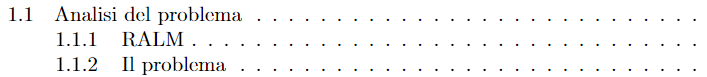
\includegraphics[width=0.8\columnwidth]{images/esempioIndice.png}
    \caption{Esempio di elementi ripetuti da minimizzare nella conversione del contenuto.}
    \label{fig:reps}
\end{figure}

\subsection{Il progetto}
Gli elementi sui quali mi sono concentrato di più per migliorare la qualità delle risposte fornite dal RALM sono state le tabelle e i titoli.
Ho applicato un metodo di conversione delle tabelle in modo tale da poterle rendere comprensibili al RALM e che potessero comunque mantenere il senso della loro struttura anche se sottoforma di testo non strutturato. \\
Per migliorare la probabilità di trovare chunk rilevanti vengono aggiunti i titoli ai chunk (ove possibile) in modo tale da potergli dare un senso di posizione all'interno del documento. \\
Le ripetizioni di caratteri vengono semplicemente ridotte a un singolo carattere.

\section{L'azienda: Siav S.p.A.}

\begin{figure}[!h] 
    \centering 
    
\includegraphics[width=0.5\columnwidth]{images/logoSiav.jpg} 
    \caption{Logo dell'azienda Siav S.p.A.}
\end{figure}
Siav S.p.A. è un’azienda informatica specializzata nella dematerializzazione, nella gestione elettronica dei documenti e nei processi digitali.
Fondata nel 1990 a Rubano (Padova) è oggi la prima azienda italiana nel settore dell’Enterprise Content Management, e offre software, soluzioni in cloud e servizi di outsourcing per la Gestione Elettronica dei Documenti, il Protocollo Informatico, il Workflow Management, la Fatturazione Elettronica e la Conservazione Digitale.



\section{Organizzazione del testo}

\begin{description}
    \item[{\hyperref[cap:analisi-preliminare]{Il secondo capitolo}}] decrive gli obiettivi nel dettaglio e mostra le varie soluzioni applicate per poter rendere migliore la qualità delle risposte del RALM;
    
    \item[{\hyperref[cap:progettazione-codifica]{Il terzo capitolo}}] approfondisce le tecnologie utilizzate nel progetto, la progettazione e la codifica di quanto sviluppato;
    
    \item[{\hyperref[cap:verifica-validazione]{Il quarto capitolo}}] illustra i vari test effettuati sul RALM e mostra i risultati ottenuti ogni modifica attuata;
    
    \item[{\hyperref[cap:conclusioni]{Nel quinto capitolo}}] vengono scritte le conclusioni riguardo al progetto svolto.
\end{description}

Riguardo la stesura del testo, relativamente al documento sono state adottate le seguenti convenzioni tipografiche:
\begin{itemize}
	\item gli acronimi, le abbreviazioni e i termini ambigui o di uso non comune menzionati vengono definiti nel glossario, situato alla fine del presente documento; 
	\item per la prima occorrenza dei termini riportati nel glossario viene utilizzata la seguente nomenclatura: \emph{parola}\glsfirstoccur;
\end{itemize}

    %\input{chapters/processi}
    \chapter{Studio e ricerca preliminare}
\label{cap:analisi-preliminare}

\intro{In questo capitolo vengono descritte nel dettaglio tutte le problematiche da risolvere durante lo sviluppo del progetto.
Verranno illustrate nel dettaglio le varie metodologie individuate per poter rendere di maggiore qualità le risposte fornite dal RALM tramite il raggiungimento dei diversi obiettivi.} \\

\section{Analisi dei requisiti}

\subsubsection{Requisiti}
\label{subsec:requisiti}
Una prima versione di backend dei servizi di estrazione di testo era già disponibile e lo scopo di questo progetto era quello di migliorare proprio quest'ultimo raggiungendo i seguenti obbiettivi:

\begin{itemize}
    \item Obbligatori:
    \subitem \gls{Parsing}\glsfirstoccur ad-hoc per documenti in cui le componenti grafiche contribuiscono alla semantica (es. tabelle e immagini);
    \subitem Estrapolazione, per alcuni formati dove sia possibile, della struttura logica del documento (es. individuando titoli e paragrafi);
    \subitem Pulizia del testo estratto dai documenti (es. eliminazione delle componenti inutili come gli indici e i sommari).
    \item Desiderabili:
    \subitem Interpretazione delle immagini allo scopo di arricchire i \gls{chunk}\glsfirstoccur in cui sono contestualizzate. 
\end{itemize}

I formati dei file considerati in questo stage sono stati i seguenti:
\begin{itemize}
    \item Pdf;
    \item Docx;
    \item HTML.
\end{itemize}

\subsection{Problematiche}
Non sempre il RALM è in grado di fornire una risposta corretta o soddisfacente.
Diverse sono state le criticità da risolvere durante lo sviluppo sia per quanto riguarda il rendere più comprensibile il contenuto al RALM, sia per quanto riguarda le conversioni dei documenti nei vari formati.
Tika, il tool utilizzato per estrarre il contenuto in testo non strutturato, durante la conversione ha delle perdite sulla struttura del contenuto come ad esempio le perdite di informazioni sulla struttura delle tabelle oppure sulla struttura del documento in sè (titolo, paragrafi, sottoparagrafi).
Per agevolare la comprensione del RALM, velocizzare le operazioni di ricerca dell'informazione e fare in modo di aumentare la probabilità che le risposte siano corrette è necessario trovare un modo per mantenere in maniera efficace queste strutture all'interno del testo semplice.
Un vantaggio di Tika è che può anche convertire il contenuto in formati strutturati come l'XHTML.
Grazie a questa funzione sarebbe già possibile individuare titoli, paragrafi e tabelle del documento ma, purtroppo, non è possibile farlo in tutti i formati: per i file HTML e Docx, dove c'è già una struttura di base, Tika riesce a identificare i vari elementi semantici, mentre con i Pdf la questione risulta più complessa.
Inoltre, non sempre, Tika riesce a ottenere la struttura esatta della tabella rispetto a come è rappresentata.
L'ultimo punto da analizzare è la questione delle ripetizioni di alcuni caratteri come segni di punteggiatura, newline e spazi: chiaramente Tika non è in grado di riconoscere quando ci sono degli elementi superflui all'interno del contenuto, è necessario quindi capire come fare per ridurre al minimo la quantità di caratteri all'interno del testo. 


\section{Ricerca e studio preliminare}
\subsection{Table Question Answering}
Nel \gls{TQA} le domande poste dall'utente cercano di avere una risposta precisa con i dati ricavati da delle tabelle.
L'obiettivo è quello di migliorare l'accesso e la comprensione delle informazioni strutturate contenute nelle tabelle.

\subsubsection{Linearizzazione delle tabelle}
\label{subsubsec-lin-tab}
Una tabella può assumere moltissime strutture e per questo è stato deciso di considerare solamente le tabelle che avessero come prima riga 
un'intesazione orizzontale e nelle righe successive i vari dati (esempio: tabella \ref{tab:esempio-cibo}).

\begin{table}[H]
    \centering
    \begin{tabular}{|p{3cm} |p{2cm} |p{2cm}| p{2cm}| p{2cm}|}
        \hline
        Cibo & Quantità & Energia(KCal) & Carboidrati(g) & Proteine(g) \\
        \hline
        Pennette rigate & 100g & 359 & 71 & 13 \\
        \hline
        Latte & 100ml & 47 & 4,9 & 3,2 \\
        \hline
        Banana & 100g & 89 & 23 & 1,1 \\
        \hline
    \end{tabular}
    \caption{Esempio di tabella presa in considerazione (valori approssimativi).}
    \label{tab:esempio-cibo}
\end{table}
\noindent Come specificato precedentemente le tabelle al momento dell'estrazione venivano linearizzate in testo semplice
perdendo alcune informazioni necessarie per la lettura effettuata dal RALM. 

\noindent Per esempio la tabella \ref{tab:esempio-cibo} verrebbe linearizzata in questa maniera:
\begin{tcolorbox}[colback=white, colframe=black]
    Cibo Quantità Energia(KCal) Carboidrati(g) Proteine(g) Pennette rigate  100g  359  71  13 Latte 100ml 47 4,9 3,2 Banana  100g 89 23 1,1
\end{tcolorbox}
\noindent La tabella linearizzata perde quindi le informazioni sulla struttura e come risultato abbiamo una serie di valori posti senza avere troppo senso in fase di lettura per un RALM. \\

\subsubsection{L'idea}
\noindent Dopo un attenta ricerca effettuata su vari documenti scientifici sono riuscito ad individuare un modo semplice ed efficace per mantenere 
l'informazione nella tabella linearizzata e la sua struttura:
\begin{itemize}
    \item All'inizio di ogni riga viene scritto "Riga n->" dove n sta per il numero della riga;
    \item Per ogni cella presente nella tabella vengono concatenati il valore dell'intestazione della colonna dov'è presente il valore e il valore della cella separati dal carattere ":";
    \item Ogni cella viene poi separata dall'altra con il carattere "|".
    \item A chiudere la riga viene inserito il carattere di escape per newline.
\end{itemize} 

Quindi la tabella \ref{tab:esempio-cibo} viene linearizzata in questo modo:
\begin{tcolorbox}[colback=white, colframe=black]
    Riga0->Cibo: Pennette rigate|Quantità:100g|Energia(KCal):359|Carboidrati(g): \\
    71|Proteine(g):13| \\
    Riga1->Cibo: Latte|Quantità:100ml|Energia(KCal):47|Carboidrati(g):4,9|\\
    Proteine(g):3,2| \\
    Riga2->Cibo: Banana|Quantità:100g|Energia(KCal):89|Carboidrati(g):23|\\
    Proteine(g):1,1|
\end{tcolorbox}

Nel metodo scritto sul seguente articolo scientifico \cite{art:multimodelqa} (paragrafo 4 \emph{Models}, sottosezione \emph{Table QA Module}) utilizza come sepratori di cella il carattare ';' e come speratore dal numero di riga alla prima cella il carattere ':'.
Ho pensato che sarebbe stato meglio utilizzare i caratteri '|', '->' per rappresentare una riga perchè sono molto meno frequenti rispoetto a quelli utilizzati nell'articolo.



\subsection{Chunking}
\paragraph{Procedimento}
Il \emph{chunking} è il procedimento mediante il quale in contenuto testuale di un documento viene suddiviso in parti più piccole chiamate chunk.
\noindent Per poter fornire una risposta ben strutturata viene utilizzato un \emph{\gls{Chat-Completion Model}}\glsfirstoccur che riceve in ingresso una richiesta e tramite quest'ultima è in grado di costruire una risposta ben strutturata.
La richiesta è formata dalla domanda dell'utente seguita dai chunk a cui il motore di ricerca ha dato lo score più alto.
Il modello in ingresso può prendere un numero limitato di \emph{token} quindi non gli si può dare l'intero contenuto del documento, ha bisogno di questa suddivisione.

\noindent Per poter capire al meglio il significato delle parole presenti in un determinato contesto è necessario dover spezzare i chunk in \emph{token}.
Il \emph{token} indica una singola unità linguistica o comunque un elemento individuale all'interno di un testo e può rappresentare per esempio una parola, un simbolo di punteggiatura o anche una parte di una parola.
Qui di seguito viene spiegato come il motore di ricerca è in grado di assegnare lo score ai vari chunk e quindi come si riesce a capire quali sono i chunk che come contenuto avranno con maggior probabilità la risposta che si sta cercando.

\subsubsection{Recupero delle informazioni}
\label{subsubsec:rec-inf}
\paragraph{\gls{BM25}}
BM25 è una ranking function usata dai motori di ricerca, è un algoritmo di tipo \emph{\gls{Bag-of-Words}}\glsfirstoccur e calcola un punteggio per ogni chunk
presente in base alla frequenza di vari termini presenti nella query di ricerca (informazioni ricavate da \cite{site:wikiOkapi}). 

\paragraph{Vector search}
Tramite la vector search vengono generate rappresentazioni vettoriali dei dati ed è possibile calcolare la similarità tra i vettori.
Per poter riconoscere il vero significato attribuito ad una parola i chunk vengono suddivisi a loro volta in token.
Grazie a questi token è possibile calcolare la distanza tra i vettori tramite.
Il tipo di distanza utilizzata in questo progetto è stata la \emph{Cosine Distance}.

\subparagraph{Cosine similarity}
La \emph{Cosine similarity} misura l'angolo tra due vettori in uno spazio multidimensionale (con l'idea che due vettori simili puntino in direzioni simili).
La cosine similarity e la cosine distance hanno una relazione inversa: all'aumentare della distanza la similarità diminuisce e viceversa.

\noindent Dati due vettori A,B la \emph{cosine similarity} viene calcolata come segue:

\[
\text{Cos(A,B)} = \frac{{\mathbf{A} \cdot \mathbf{B}}}{{\|\mathbf{A}\| \cdot \|\mathbf{B}\|}}    
\]

\[
\text{Cosine distance} = 1-Cos(A,B)
\]

\noindent (Informazioni ricavate da \cite{site:weaviate-distance-metrics}).

\paragraph{Ricerca ibrida}
Il tipo di ricerca applicata in Weaviate per questo progetto è stata la ricerca ibridia che sfrutta sia BM25 che la \emph{Vector search} per poter stabilire uno score per i chunk.

\subparagraph{\gls{RRF}}
L'RRF score è il calcolo attreverso il quale riusciamo ad avere uno score unico per la ricerca ibrida.
Ad ogni documento viene assegnato un punteggio che equivale alla somma dei reciproci dei suoi piazzamenti nelle varie ranked list ottenute tramite gli altri algoritmi utilizzati nella ricerca.

\[
\text{RFF} = \sum_{d \in D} (\frac{1}{k+r(d)})    
\]

\noindent Per esempio, nella tabella \ref{tab:ranking}, vengono dati tre chunk A, B, C e vengono classificati nella seguente maniera tramite i due ranking algorithm:

\begin{table}[H]
    \centering
    \begin{tabular}{|p{2cm} |p{2cm} |p{2cm}|}
        \hline
        Posizione & BM25 & Vector Search \\
        \hline
        1 & A & B \\
        \hline
        2 & B & C \\
        \hline
        3 & C & A \\
        \hline
    \end{tabular}
    \caption{Esempio di ranking per i documenti A, B, C tramite BM25 e Vector Search.}
    \label{tab:ranking}
\end{table}

\noindent Gli RRF score dei documenti A, B, C sono i seguenti:
\begin{table}[H]
    \centering
    \begin{tabular}{|p{3cm} | p{3cm} |}
        \hline
        Chunk & RRF score \\
        \hline
        A & 1/1 + 1/3 = 1.3\\
        \hline
        B & 1/2 + 1/1 = 1.5\\
        \hline
        C & 1/3 + 1/2 = 0.83\\
        \hline
    \end{tabular}
    \caption{Esempio di calcolo del RRF score per i documenti A, B, C.}
    \label{tab:hybridrank}
\end{table}

\noindent Nella tabella \ref{tab:hybridrank} abbiamo quindi che il miglior chunk da considerare è il chunk B seguito poi dal chunk A e dal C.\\
\\
\noindent (Informazioni ricavate da \cite{site:weaviate-hybrid-search}).

\subsubsection{L'idea}
\label{subsubsec:ideachunking}
Per migliorare la qualità del chunking sono state attuate due strategie:
\begin{itemize}
    \item Il chunk viene strutturato come segue: all'inizio sarà presente una lista di titoli consevutivi in ordine gerarchico per individuare il contesto del chunk. In base alla grandezza del chunk viene definita una quantità di token che definisce la lunghezza della lista dei titoli. Se questa grandezza viene superata si scarta il titolo più alto in ordine gerarchico fino a quando i token effettivi saranno minori rispetto alla quantità prestabilita.
    La grandezza scelta per la lista dei titoli equivale ai due ottavi della grandezza del chunk mentre il resto viene lasciato per il contenuto.
    \noindent Il contenuto del paragrafo viene concatenato separando le tabelle dal testo:
    \begin{itemize}
        \item Se viene trovata una tabella si cerca di inserire le intere righe all'interno del chunk in modo tale da non perdere informazioni sui dati;
        \item Se viene trovato del testo normale viene utilizzata la sliding window per inserire parte del contenuto del chunk precedente all'inzio del nuovo chunk.
    \end{itemize}

    Quando viene utilizzata la sliding window quindi si creerà l'\emph{\gls{overlap}}\glsfirstoccur del contenuto.
    L'overlap è utile per due motivi:
    \begin{itemize}
        \item Se ci sono n chunk consecutivi nella lista dei chunk migliori è possibile unirli in modo deterministico, inoltre anche il modello è in grando di riconoscere questa continuità;
        \item Senza di esso ci sarebbero delle frasi spezzate prive di significato all'interno dei chunk.
    \end{itemize}

    Come esempio un documento potrebbe avere la seguente struttura:
    \begin{tcolorbox}[colback=white, colframe=black]
        1 Titolo\\
        testo\\
        tabella\\
        1.1 Sottotitolo\\
        testo\\
        1.1.1 Sottotitolo\\
        testo\\
        1.1.2 Sottotitolo\\
        testo\\
    \end{tcolorbox}

    Assumiamo che ogni titolo è composto da 1 token, ogni componente testuale è composta da 6 token e ogni riga della tabella da 5 token. Il chunk può essere composto al massimo da 8 token.
    \begin{tcolorbox}[colback=white, colframe=black]
        \begin{itemize}
            \item Chunk1: 1 Titolo:testo (7 token)
            \item Chunk2: 1 Titolo: prima riga della tabella (6 token)
            \item Chunk3: 1 Titolo: seconda riga della tabella (6 token)
            \item Chunk4: 1 Titolo| 1.1 Sottotitolo: testo (8 token)
            \item Chunk5: 1.1 Sottotitolo | 1.1.1 Sottotitolo: testo (8 token -> Qui viene eliminato "1 Titolo" perchè sennò si sforerebbe la grandezza prestabilita)
            \item Chunk6: 1.1 Sottotitolo | 1.1.2 Sottotitolo: testo (8 token -> Come nel chunk precedente viene eliminato "1 Titolo")
        \end{itemize}
    \end{tcolorbox}
    
    \item Pulizia del testo: le serie di caratteri  (come spazi, newline, '-', '*', altro), scelti prima di effettuare la pulizia, vengono sostituiti con un unico carattere dello stesso tipo.
    \noindent Ogni carattere è composto da un singolo token e quindi i chunk nel caso in cui non si eliminassero queste ripetizioni avrebbero dei caratteri superflui che occuperebbero spazio inutilmente, ci sarebbe il rischio di creare più chunk del dovuto.  
\end{itemize}

\section{Pianificazione del lavoro}
Le attività per sviluppare il lavoro e le ore previste per ognunga di esse sono riportate nella tabella successiva.
Come si può notare dal diagramma di Gantt diverse attività si sovrappongono e questo accade perchè diverse di queste ultime hanno dei punti in comune. 

\subsection{Pianificazione delle attività}
\begin{table}[H]
    \centering
    \begin{tabular}{p{2cm} p{8cm} p{2cm}}
        \hline
        Numero attività & Attività & Ore previste \\
        \hline
        1 & Studio introduttivo su Natural Language Processing e Large Language Model & 16 \\
        \hline
        2 & Studio delle tecniche di estrazione di testo e dei principali tool nell'ambito dell'NLP & 16 \\
        \hline
        3 & Studio dell'attuale implementazione del chatbot basato su retrueval-augmented LLM & 16 \\
        \hline
        4 & Analisi dei requisiti con studio delle casistiche da gestire & 30 \\
        \hline
        5 & Progettazione delle varie componenti richieste nel paragrafo  & 70 \\
        \hline
        6 & Implementazione del software & 100 \\
        \hline
        7 & Test e sperimentazione del software & 24 \\
        \hline
        8 & Documentazione & 48 \\
        \hline
    \end{tabular}
    \caption{Tabella di pianificazione delle attività.}
    \label{tab:preventivo}
\end{table}

\subsection{Diagramma di Gantt delle attività}
Viene mostrato il diagramma di Gantt delle attività svolte durante le nove settimane dello stage.

\begin{figure}[H]
    \centering
    \begin{ganttchart}[
        expand chart=\textwidth,
        hgrid=true,
        vgrid=true
        ]{1}{9}
        \gantttitlelist{1,...,9}{1} \\
        \ganttbar{Studio NLP e LLM}{1}{1} \\
        \ganttbar{Studio tecniche e tool esistenti}{1}{2} \\
        \ganttbar{Studio attuale implementazione chatbot}{2}{2} \\
        \ganttbar{Analisi dei requisiti}{2}{3} \\
        \ganttbar{Progettazione}{3}{5} \\
        \ganttbar{Implementazione del software}{5}{8} \\
        \ganttbar{Test e sperimentazione del software}{8}{9} \\
        \ganttbar{Documentazione}{1}{9} 
    \end{ganttchart}
    \caption{Diagramma di Gantt delle attività.}
\end{figure}




    %\chapter{Analisi dei requisiti}
\label{cap:analisi-requisiti}

\intro{Breve introduzione al capitolo}\\

\section{Casi d'uso}

Per lo studio dei casi di utilizzo del prodotto sono stati creati dei diagrammi.
I diagrammi dei casi d'uso (in inglese \emph{Use Case Diagram}) sono diagrammi di tipo \gls{uml} dedicati alla descrizione delle funzioni o servizi offerti da un sistema, così come sono percepiti e utilizzati dagli attori che interagiscono col sistema stesso.
Essendo il progetto finalizzato alla creazione di un tool per l'automazione di un processo, le interazioni da parte dell'utilizzatore devono essere ovviamente ridotte allo stretto necessario. Per questo motivo i diagrammi d'uso risultano semplici e in numero ridotto.


\begin{usecase}{0}{Scenario principale}
\usecaseactors{Sviluppatore applicativi}
\usecasepre{Lo sviluppatore è entrato nel plug-in di simulazione all'interno dell'IDE}
\usecasedesc{La finestra di simulazione mette a disposizione i comandi per configurare, registrare o eseguire un test}
\usecasepost{Il sistema è pronto per permettere una nuova interazione}
\label{uc:scenario-principale}
\end{usecase}

\section{Tracciamento dei requisiti}

Da un'attenta analisi dei requisiti e degli use case effettuata sul progetto è stata stilata la tabella che traccia i requisiti in rapporto agli use case.\\
Sono stati individuati diversi tipi di requisiti e si è quindi fatto utilizzo di un codice identificativo per distinguerli.\\
Il codice dei requisiti è così strutturato R(F/Q/V)(N/D/O) dove:
\begin{enumerate}
	\item[R =] requisito
    \item[F =] funzionale
    \item[Q =] qualitativo
    \item[V =] di vincolo
    \item[N =] obbligatorio (necessario)
    \item[D =] desiderabile
    \item[Z =] opzionale
\end{enumerate}
Nelle tabelle \ref{tab:requisiti-funzionali}, \ref{tab:requisiti-qualitativi} e \ref{tab:requisiti-vincolo} sono riassunti i requisiti e il loro tracciamento con gli use case delineati in fase di analisi.

\newpage

\begin{table}%
\caption{Tabella del tracciamento dei requisti funzionali}
\label{tab:requisiti-funzionali}
\begin{tabularx}{\textwidth}{lXl}
\hline\hline
\textbf{Requisito} & \textbf{Descrizione} & \textbf{Use Case}\\
\hline
RFN-1     & L'interfaccia permette di configurare il tipo di sonde del test & UC1 \\
\hline
\end{tabularx}
\end{table}%

\begin{table}%
\caption{Tabella del tracciamento dei requisiti qualitativi}
\label{tab:requisiti-qualitativi}
\begin{tabularx}{\textwidth}{lXl}
\hline\hline
\textbf{Requisito} & \textbf{Descrizione} & \textbf{Use Case}\\
\hline
RQD-1    & Le prestazioni del simulatore hardware deve garantire la giusta esecuzione dei test e non la generazione di falsi negativi & - \\
\hline
\end{tabularx}
\end{table}%

\begin{table}%
\caption{Tabella del tracciamento dei requisiti di vincolo}
\label{tab:requisiti-vincolo}
\begin{tabularx}{\textwidth}{lXl}
\hline\hline
\textbf{Requisito} & \textbf{Descrizione} & \textbf{Use Case}\\
\hline
RVO-1    & La libreria per l'esecuzione dei test automatici deve essere riutilizzabile & - \\
\hline
\end{tabularx}
\end{table}%

    \chapter{Progettazione e codifica}
\label{cap:progettazione-codifica}

\intro{Breve introduzione al capitolo}\\

\section{Tecnologie e strumenti}
\label{sec:tecnologie-strumenti}

Di seguito viene data una panoramica delle tecnologie e degli strumenti utilizzati per sviluppare il progetto.
\subsection{Python}
Python offre diverse librerie utili per l'apprendimento automatico, il trattamento del linguaggio naturale e molto altro ancora.
\subsection{Jupiter Notebook}
Applicazione che permette di creare documenti testuali contenenti anche codice eseguibile. Utile per realizzare e documentare analisi di dati.
\subsection{Tika}
\label{subsec:tika}
Tika è un tool che permette di estrarre dai file i suoi metadata (come titolo del file, autore e altro) e il suo contenuto sottoforma di testo (strutturato e non).
Riesce ad estrarre i dati da molti formati tra cui Pdf, docx e html.
\subsection{Pandas}
\label{subsec:pandas}
Pandas è una libreria che fornisce strutture dati e strumenti per la manipolazione e l'analisi dei dati.
Il primo passo importante dell'estrazione delle tabelle dai vari documenti è stato quello di avere un DataFrame a disposizione con i valori di quest'ultime. 
Pandas è stato utilizzato per l'estrazione delle tabelle dai file in formato html e docx.
\subsection{PdfPlumber}
\label{subsec:pdfplumber}
PdfPlumber è una libreria per Python che fornisce funzionalità per l'estrazione automatizzata di testo e tabelle dai documenti PDF.
Nel progetto è stato utilizzato per estrarre le tabelle dai vari pdf.
\subsection{Python-docx}
\label{subsec:python-docx}
Python-docx è una libreria che consente di creare, modificare e leggere documenti Microsoft Word.
Grazie a questa libreria è possibile manipolare le tabelle presenti all'interno dei file docx.
\subsection{BeautifulSoup}
\label{subsec:beautifulsoup}
BeautifulSoup è una libreria Python che facilita l'estrazione di dati da file HTML e XML.
Consente, inoltre, di creare e modificare tag all'interno del codice con il quale si sta lavorando.
\subsection{OpenAI API}
API fornita da OpenAI tramite la quale si possono sfruttare i vari modelli offerti per la generazione di testo in linguaggio naturale.
\subsection{Weaviate}
\label{subsec:weav}
Weaviate è un database vettoriale utile per la ricerca dei dati basata sulla loro semantica e sulle loro relazioni. 

\section{Progettazione e codifica}
\label{sec:progettazione-codifica}
La parte di codice sviluppata per questo progetto integra la parte di logica dell'applicazione di un backend già esistente.

\begin{figure}[!h]
    \centering
    \scalebox{0.5}{
        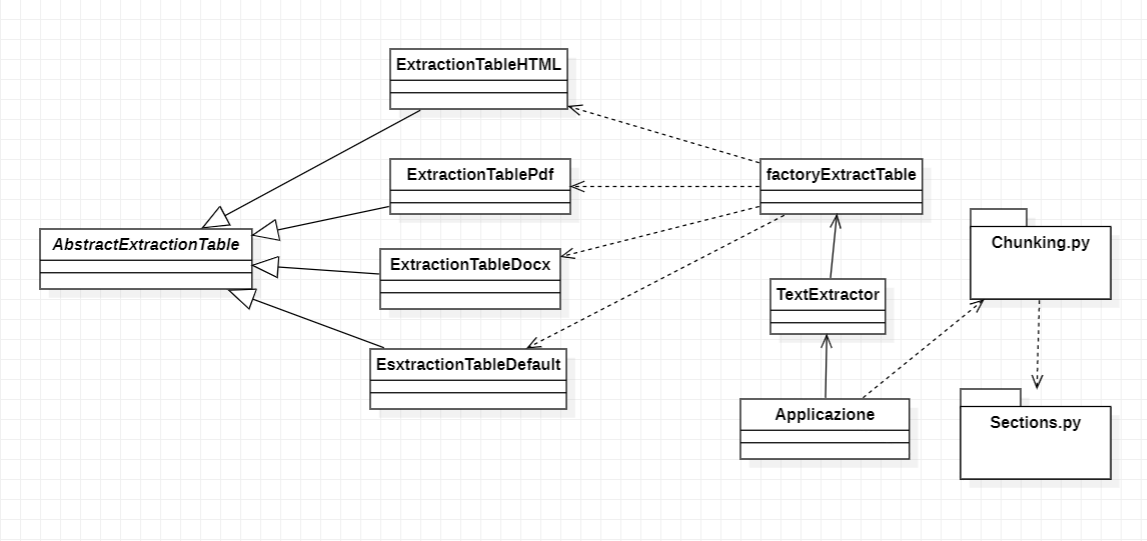
\includegraphics{images/architettura.png}
    }
    \caption{Architettura della parte di codice implementata nel backend}
\end{figure}

\subsection{L'idea}
Grazie a Tika riusciamo a convertire il contenuto dei documneti in XHTML in modo tale da poter lavorare con del testo strutturato.
Con i documenti dove c'è già una struttura al di sotto Tika riesce a convertire molto bene il contenuto dei documenti in un XHTML ed è in grado di individuare intestazioni (e i loro livelli gerarchici h1,h2,...), tabelle e altro.
Per questo non è stato difficile riuscire a implementare le funzioni utili per lavorare con i file HTML e Docx.
Per i Pdf invece le cose sono state più complesse, gli unici tool individuati che riescono a convertire bene il contenuto dei pdf (come "Aspose") in testo strutturato richiedono una licenza a pagamento e quindi è stato utilizzato comunque Tika.
In questo caso il contenuto viene rappresentato tramite dei tag \emph{div} che rappresentano le singole pagine e il contenuto stesso viene trascritto tramite dei tag \emph{p}. \\

\noindent Qui di seguito vengono descritte le parti di codice sviluppate di maggiore rilevanza.

\subsection{ExtractionTable}
ExtractionTableHTML, ExtractionTableDocx, ExtractionTablePdf e ExtractionTableDefault implementano la classe AbstractExtractionTable ed espongono quelle funzioni utili alle operazioni da fare sulle tabelle presenti nei documenti di quello specifico formato:
\begin{itemize}
    \item La funzione \textbf{extractTable} prende in ingresso un file path e restituisce la lista delle tabelle, convertite in DataFrame, presenti nel documento indicato nel percorso. Per estrarre le tabelle sono stati utilizzati i seguenti tool:
    \begin{itemize}
        \item HTML: \nameref{subsec:pandas};
        \item Docx: \nameref{subsec:python-docx};
        \item Pdf: \nameref{subsec:pdfplumber};
    \end{itemize}
    \item La funzione \textbf{replaceTable} prende in ingresso un file path, una lista di tabelle da sostituire all'interno del documento e ritorna la versione XHTML del documento estratta tramite \nameref{subsec:tika} con le tabelle linearizzate sostituite all'interno.
    Per HTML e Docx la funzione rimane uguale: grazie a \nameref{subsec:beautifulsoup} è possibile cercare tutti i vari tag \emph{table} e sostituire il loro contenuto. Per i Pdf invece sono state usate le espressioni regolari per cercare e sostituire le tabelle. 
    \item Le tabelle vengono linearizzate tramite la funzione \textbf{adaptTable} che prende in ingresso un DataFrame e ritorna la stringa che rappresenta la tabella.
\end{itemize} 

\subsection{FactoryExtractTable}
Viene presentata una funzione \textbf{factoryExtractTable} che prende in ingresso un file path e in base al suo formato istanzia un oggetto di tipo ExtractionTable.
Quando viene inserito un file in un formato che non corrisponde a uno dei tre principali viene instanziato un oggetto di tipo ExtractionTableDefault.
Si è deciso di sviluppare questa classe per avere comunque delle possibilità nella sostituizione delle tabelle nel caso in cui si riesce a convertire discretamente il documento in XHTML.

\subsection{TextExtractor}
TextExtractor mette a disposizione la funzione \textbf{extractText} che prende in ingresso un file path e un booleano \emph{getText}.
Questa funzione ritorna:
\begin{itemize}
    \item Con getText = False, il contenuto del documento convertito in XHTML;
    \item Con getText = True, il contenuto del documento convertito il stringa (testo non strutturato). 
\end{itemize}

Per lavorare più facilmente con il contenuto XHTML prodotto dalla conversione dei pdf, al \emph{body} viene aggiunto un primo titolo \emph{h1} con contenuto il nome del file come primo tag e vengono estratti tutti i tag da dentro i \emph{div} che rappresentano le pagine (individuabili con BeautifulSoup perchè hanno \emph{"class=page"}).

\subsection{Sections.py}
Modulo creato che contiene funzioni utili per convertire un XHTML in una struttura ad albero rinominata "Sezione"

La Sezione viene definita in base ai vari titoli dei paragrafi e al loro livelo gerarchico ed è formata dai seguenti campi:
\begin{itemize}
    \item titolo (stringa): titolo della sezione;
    \item contenuto (lista): all'interno della lista ci può essere sia contenuto testuale che altre sezioni. 
\end{itemize}

La funzione che viene esposta per creare la Sezione si chiama \textbf{makeSection} e prende in ingresso contenuto in forma XHTML.

\subsection{Chunking.py}
Modulo creato che contiene funzioni utili per la conversione delle Sezione in Chunk.

Il Chunk è formato dai seguenti campi:
\begin{itemize}
    \item titolo (stringa): titolo della chunk;
    \item parentsTit (lista di stringhe): contiene tutti i titoli superiori in senso gerarchico al paragrafo;
    \item contenuto (stringa): porzione di contenuto del paragrafo.
    \item page (intero): numero della pagina da dove è stato preso il contenuto del chunk (ancora non utilizzato, messo per successivi aggiornamenti del codice). 
\end{itemize}

Le funzioni esposte e utili all'esterno di questo modulo sono le seguenti:
\begin{itemize}
    \item La funzione \textbf{chunking} che prende in ingresso il contenuto XHTML di un documento, il numero massimo di token da cui può essere composto un chunk, la funzione di encode da testo in token e la funzione di decode da token a testo.
    Questa funzione sfrutta makeSection (definita in Section.py) e restituisce la lista ordinata di chunk che compongono il documento.
    All'interno della funzione viene chiamata anche la funzione \textbf{cleanText} effettua la pulizia del testo rimuovendo le ripetizioni dei caratteri passati come input.
    \item La funzione \textbf{createTitleForChunk} crea la stringa di titoli unita in base a un numero massimo di token da cui può essere composta, prende una lista di titoli e il numero di token che possono comporre la stringa.
    Questa funzione non ha senso di essere applicata sui documenti nei quali Tika non riesce a riconoscere una struttura: viene trovato un unico titolo che è il nome del file e sostanzialmente è come se fosse tutto sotto un unico paragrafo.
\end{itemize}

\subsection{Applicazione}
La parte dell'applicazione effettiva in questo momento è implementata tramite un Jupiter Notebook ed è il prototipo che mi è stato passato all'inizio dello stage.
Quello che ho fatto è stato chiamare le varie funzioni per ottenere le tabelle linearizzate e il chunking migliorato all'interno.
La procedura che viene eseguita per far funzionare il prototipo è la seguente:
\begin{enumerate}
    \item Viene dato un insieme di documenti;
    \item Ogni documento convertito in XHTML tramite \textbf{extractText} che a sua volta linearizza le tabelle;
    \item Vengono creati i chunk tramite la funzione \textbf{chunking};
    \item I vari chunk vengono caricati sul motore di ricerca;
    \item Quando viene posta una domanda, vengono restituiti i 10 chunk con lo score più alto (hybrid search);
    \item La richiesta (domanda + 10 chunk) viene consegnata al Chat-Completion Model che elabora le informazioni e restituisce una risposta alla domanda. 
\end{enumerate}

\section{Design pattern}

Per strutturare il codice in maniera tale da renderlo di facile manutenzione ed estensione sono stati usati i \gls{design pattern}\glsfirstoccur.
Il design pattern utilizzato è stato lo \textbf{\gls{strategy}}\glsfirstoccur: per ogni formato dei file l'estrazione della tabella avviene in maniera differente quindi viene applicato lo strategy pattern che definisce una classe astratta \emph{AbstractExtractionTable} che verrà poi implementata a seconda del formato preso in cosiderazione. 

    \chapter{Verifica e validazione}
\label{cap:verifica-validazione}

\intro{In questo capitolo vengono riportati tutti i dati e le prove effettuate sul RALM per ogni modifica aggiunta}

\section{Test}
Come fonte di informazioni per il RALM sono state scelte cinque pagine di Wikipedia e sono state convertite nei formati desiderati (HTML, Pdf, Docx).
La pagine scelte sono composte di testo e altri elementi semantici, tra cui le tabelle che hanno la struttura della tabella \ref{tab:esempio-cibo} spiegata nel paragrafo \nameref{subsubsec-lin-tab}

I test sono stati effettuati tramite una valutazione umana secondo i seguenti criteri:
\begin{itemize}
    \item La risposta deve essere ben strutturata, scritta in maniera corretta e comprensibile;
    \item La risposta deve essere corretta e completa.
\end{itemize}

Sulla base di ciò a ogni risposta viene assegnato un valore tra 0 (risposta non corretta/strutturata male) e 1 (risposta corretta e strutturata correttamente)

\subsection{Domande}
Sono stati creati due set da 10 domande l'uno, le domande sono state create in maniera tale da poter interrogare il modello sui dati presenti nelle tabelle dei vari documenti:
\begin{itemize}
    \item Set di domande semplici: domande che interrogano il RALM su singole celle delle tabelle o celle che hanno la stessa intestazione;
    \item Set di domande complesse: domande che interrogano il RALM su diverse celle e che chiedono di fare diverse operazioni tra i dati presenti (es: somma, media).
\end{itemize}

\subsubsection{Set di domande semplici}
\begin{table}[H]
    \centering
    \begin{tabular}{|p{0.5cm} |p{2.5cm} |p{4cm}| p{4.5cm}|}
        \hline
        \textbf{N}. & \textbf{Nome pagina} & \textbf{Domanda} & \textbf{Risposta corretta} \\
        \hline
        1 & Italia & Quali sono le 3 città italiane con più abitanti? & Roma, Milano, Napoli \\
        \hline
        2 & Italia & Nel settore terziario italiano, qual è il settore che presenta più imprese? & Il commercio \\
        \hline
        3 & Avanti un altro! & In quali paesi è stato esportato Avanti un altro? & Spagna, Albania, Ungheria, Vietnam, Brasile, Bulgaria, Cile, Paraguay, Canada, Turchia, Polonia, Romania \\
        \hline
        4 & Avanti un altro! & In che canale è stato trasmesso Avanti un altro? & Canale 5\\
        \hline
        5 & SPAR & In che anno è arrivato SPAR in italia? & 1959 \\
        \hline
        6 & SPAR & Quanto volume d'affari ha SPAR in Belgio & 626.307 \\
        \hline
        7 & The Space Cinema & Quante sale ha il The Space Cinema di Padova? & 14 \\
        \hline
        8 & The Space Cinema & Quanti posti a sedere ha il The Space Cinema di Parma centro & 1402 \\
        \hline
        9 & Sonic(serie) & In che anno è uscito il videogioco "Sonic Battle"? & 2003 \\
        \hline
        10 & Sonic(serie) & Dov'è apparso Tails per la prima volta? & Sonic the hedghog 2 \\
        \hline
    \end{tabular}
    \caption{Set di domande semplici poste al RALM}
\end{table}

\subsubsection{Set di domande complesse}
\begin{table}[H]
    \centering
    \begin{tabular}{|p{0.5cm} |p{2.5cm} |p{4cm}| p{4.5cm}|}
        \hline
        \textbf{N}. & \textbf{Nome pagina} & \textbf{Domanda} & \textbf{Risposta corretta} \\
        \hline
        1 & Italia & Quali città hanno più di 500000 abitanti in italia? & Roma, Milano, Napoli, Torino, Palermo e Genova \\
        \hline
        2 & Italia & Quali sono le città italiane che hanno più 300000 abitanti ma meno di 387841? & Firenze, Bari, Catania \\
        \hline
        3 & Avanti un altro! & Mediamente quanti telespettatori ci sono stati per ogni edizione di avanti un altro? & circa 3700000 \\
        \hline
        4 & Avanti un altro! & Quante puntate ci sono state di avanti un altro in tutto? & Circa 1400 \\
        \hline
        5 & SPAR & In quali paesi è arrivato SPAR dal 2000 in poi? & Russia, Mauritius, Cipro, Ucraina, Cina, Croazia \\
        \hline
        6 & SPAR & In quali paesi le strutture SPAR hanno meno di 10000 metri quadrati di superficie? & Croazia, Mauritious, Zambia,  India, Albania \\
        \hline
        7 & The Space Cinema & Quali sono i the space situati in provincia di Torino? & Beinsasco, Torino - Parco Dora \\
        \hline
        8 & The Space Cinema & Quali sono i the space con più di 13 sale? & Limena, Roma Paroc de' Medici,  Vimercate \\
        \hline
        9 & Sonic(serie) & Chi è eggman e quando ha fatto la sua prima apparizione? & Eggman è un uomo esperto di ingegneria robotica che vuole conquistare il mondo di Sonic, antagonista principale della serie. Ha fatto la sua prima apparizione in "Sonic the hedghog". \\
        \hline
        10 & Sonic(serie) & Elenca tutti i giochi mobile di Sonic dal 2015 in poi & Sonic runners, sonic dash 2: sonic boom, sonic runners adventure, sonic forces speed battle, sonic speed simulaor \\
        \hline
    \end{tabular}
    \caption{Set di domande complesse poste al RALM}
\end{table}

Nei seguenti paragrafi vengono riportate le risposte del RALM a ogni aggiornamento significativo del codice per denotare l'effettivo miglioramento della qualità delle risposte:

\begin{enumerate}
    \item Prima versione: estrazione del contenuto semplice (senza linearizzazione delle tabelle, senza correzione del chunking e pulizia del testo);
    \item Seconda verione: estrazione del contenuto con la linearizzazione delle tabelle;
    \item Terza versione: estrazione del contenuto con la linearizzazione delle tabelle e la correzione del chunking;
    \item Quarta versione: estrazione del contenuto con la linearizzazione delle tabelle, correzione del chunking e pulizia del testo;

\end{enumerate}


\subsection{Test sui file HTML}

\subsubsection{Prima versione - Risposte al set di domande semplici}

\begin{table}[H]
    \centering
    \begin{tabular}{|p{0.5cm} |p{6cm} |p{2cm}|}
        \hline
        \textbf{N}. & \textbf{Risposta fornita dal RALM} & \textbf{Valutazione} \\
        \hline
        1 & Roma, Milano e Napoli sono le tre città italiane con più abitanti. & 1 \\
        \hline
        2 & Il settore che presenta più imprese nel terziario italiano è il settore dei servizi. & 0 \\
        \hline
        3 & Avanti un altro! è stato esportato in Spagna, Albania, Ungheria, Vietnam, Brasile, Paraguay, Cile, Bulgaria, Canada, Turchia, Polonia e Romania. & 1 \\
        \hline
        4 & Avanti un altro è stato trasmesso sul canale 5. & 1 \\
        \hline
        5 & SPAR è arrivato in Italia nel 1959. & 1 \\
        \hline
        6 &  SPAR in Belgio & 0 \\
        \hline
        7 & Il the space di Padova ha 14 sale & 1 \\
        \hline
        8 & Il The Space di Parma Centro ha 7 sale e 1402 posti a sedere & 1 \\
        \hline
        9 & Il videogioco Sonic Battle è stato pubblicato da Sega nel 2003. & 1 \\
        \hline
        10 & Tails è un compagno di Sonic che appare per la prima volta in Sonic the Hedgehog 2 nel 1992. & 1 \\
        \hline
    \end{tabular}
    \caption{Risposte al set di domande semplici date dalla prima versione del RALM (File HTML)}
\end{table}

\textbf{Correttezza:} 8/10

\subsubsection{Prima versione - Risposte al set di domande complesse}

\begin{table}[H]
    \centering
    \begin{tabular}{|p{0.5cm} |p{6cm} |p{2cm}|}
        \hline
        \textbf{N}. & \textbf{Risposta fornita dal RALM} & \textbf{Valutazione} \\
        \hline
        1 & Palermo, Cagliari, Trento, Venezia, Trieste, Bologna, Firenze, Perugia, Ancona, Roma, Napoli, Bari, Potenza, Catanzaro, Matera, Belluno & 0 \\
        \hline
        2 & Napoli, Palermo, Genova, Bologna, Firenze e Bari. & 0 \\
        \hline
        3 & In media si contano 3.995.000 spettatori per edizione. & 0.8 \\
        \hline
        4 & 17 edizioni, con una puntata speciale & 0 \\
        \hline
        5 & SPAR è arrivata in Belgio, Danimarca, Francia, Germania, Irlanda, Italia, Lituania, Paesi Bassi, Polonia, Regno Unito, Russia, Sudafrica, Spagna, Svizzera, Ungheria, Zimbabwe. & 0 \\
        \hline
        6 & SPAR è presente in Croazia, Slovenia, Austria, Germania, Regno Unito, Italia, Sudafrica, Norvegia, Giappone, Cina e Croazia. & 0 \\
        \hline
        7 & The Space Cinema è una catena di cinema presente in provincia di Torino. Ha 8 sale e 1295 posti a sedere. & 0 \\
        \hline
        8 & The Space Cinema è una delle catene di cinema più grandi in Italia, con 34 diverse strutture e 347 sale.  & 0 \\
        \hline
        9 & Eggman è un personaggio che è appena comparso nella serie Sonic. È uno scienziato malvagio che cerca di conquistare il mondo. & 0 \\
        \hline
        10 & Sonic mobile games from 2015 onwards: Sonic Jump (2015), Sonic Dash (2013), Sonic Jump Fever (2014), Sonic Runners (2015), Sonic Dash 2: Sonic Boom (2015), Sonic Runners Adventure (2017), Sonic Forces: Speed Battle (2017), Sonic Speed Simulator (2022) & 0 \\
        \hline
    \end{tabular}
    \caption{Risposte al set di domande complesse date dalla prima versione del RALM (File HTML)}
\end{table}

\textbf{Correttezza:} 0.8/10

\subsubsection{Seconda versione - Risposte al set di domande semplici}

\begin{table}[H]
    \centering
    \begin{tabular}{|p{0.5cm} |p{6cm} |p{2cm}|}
        \hline
        \textbf{N}. & \textbf{Risposta fornita dal RALM} & \textbf{Valutazione} \\
        \hline
        1 & Roma, Milano e Napoli sono le prime tre città italiane per popolazione. & 1 \\
        \hline
        2 & Il commercio è il settore che presenta più imprese in Italia, seguito da turismo, trasporti e logistica, e altri servizi. & 1 \\
        \hline
        3 & Avanti un altro! è stato esportato in Spagna, Albania, Ungheria, Vietnam, Brasile, Paraguay, Cile, Bulgaria, Canada, Turchia, Polonia e Romania. & 1 \\
        \hline
        4 & Avanti un altro è stato trasmesso sul canale 5. & 1 \\
        \hline
        5 & SPAR è arrivato in Italia nel 1959. & 1 \\
        \hline
        6 & SPAR ha un volume d'affari di 626.307 migliaia di € in Belgio. & 1 \\
        \hline
        7 & Il the space di Padova ha 14 sale & 1 \\
        \hline
        8 & The Space Cinema di Parma Centro ha 1402 posti a sedere. & 1 \\
        \hline
        9 & Il videogioco Sonic Battle è uscito nel 2003. & 1 \\
        \hline
        10 & Tails ha fatto la sua prima apparizione in Sonic the Hedgehog 2 (8-bit) nel 1992. Da allora, è apparso in un totale di 56 giochi. & 1 \\
        \hline
    \end{tabular}
    \caption{Risposte al set di domande semplici date dalla seconda versione del RALM (File HTML)}
\end{table}

\textbf{Correttezza:} 10/10

\subsubsection{Seconda versione - Risposte al set di domande semplici}

\begin{table}[H]
    \centering
    \begin{tabular}{|p{0.5cm} |p{6cm} |p{2cm}|}
        \hline
        \textbf{N}. & \textbf{Risposta fornita dal RALM} & \textbf{Valutazione} \\
        \hline
        1 & Le città italiane con più di 500.000 abitanti sono Milano, Roma, Torino, Palermo, Napoli e Genova. & 1 \\
        \hline
        2 & Firenze, Bari, Catania & 1 \\
        \hline
        3 & Non è chiaro quanto sia l'edizione di Avanti un altro, ma si stima che ci siano stati 3 milioni di telespettatori per edizione. & 0 \\
        \hline
        4 & In totale, ci sono stati 1.143 episodi di "Avanti un altro!" trasmessi dal 2011 al 2020. & 0 \\
        \hline
        5 & I Paesi in cui è arrivato SPAR dal 2000 in poi sono Russia, Mauritius, Cipro, Ucraina, Cina e Croazia. & 1 \\
        \hline
        6 & I paesi in cui le strutture SPAR hanno meno di 10000 metri quadrati di superficie sono la Polonia, l'Australia, l'Ucraina, la Croazia e lo Zimbabwe. & 0 \\
        \hline
        7 & I nomi dei the space situati in provincia di Torino sono Montesilvano, Napoli, Nola, Parma Campus, Parma Centro e Pradamano. & 0 \\
        \hline
        8 & I cinema The Space con più di 13 sale sono: Rozzano, Salerno, Sestu, Silea. & 0 \\
        \hline
        9 & Eggman è un personaggio che appare nella serie Sonic. È un uomo esperto di ingegneria robotica che vuole conquistare il mondo di Sonic. Ha fatto la sua prima apparizione in Sonic the Hedgehog nel 1991.  & 1 \\
        \hline
        10 & I giochi mobile di Sonic dal 2015 in poi sono: Sonic runners (2015), Sonic Dash 2: Sonic Boom (2015), Sonic Runners Adventure (2017), Sonic Forces: Speed Battle (2017) e Sonic Speed Simulator (2022). & 1 \\
        \hline
    \end{tabular}
    \caption{Risposte al set di domande complesse date dalla seconda versione del RALM (File HTML)}
\end{table}

\textbf{Correttezza:} 5/10

\subsubsection{Grafico Risposte corrette su versione}
Qui di seguito c'è il grafico che evidenzia l'andamento della quantità delle risposte corrette che vengono date dal RALM nelle sue varie versioni.


    
\begin{figure}
    
    \centering
    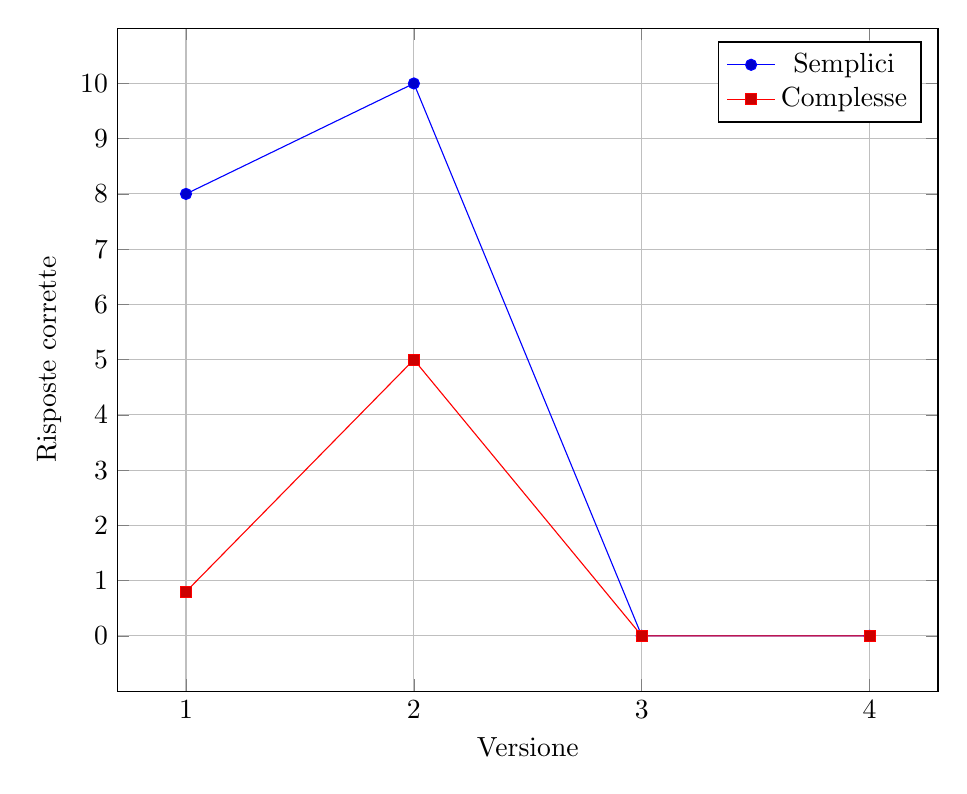
\begin{tikzpicture}
        \centering
        \begin{axis}[
            xlabel={Versione},
            ylabel={Risposte corrette},
            grid=major,
            width=12cm,
            height=10cm,
            xtick={1, 2, 3, 4}, 
            ytick={0, 1, 2, 3, 4, 5, 6, 7, 8, 9, 10}
        ]
        \addplot coordinates {
            (1, 8)
            (2, 10)
            (3, 0)
            (4, 0)
        };
        \addlegendentry{Semplici}

        \addplot coordinates {
            (1, 0.8)
            (2, 5)
            (3, 0)
            (4, 0)
        };
        \addlegendentry{Complesse}
        
        \end{axis}
    \end{tikzpicture}
    \caption{Grafico risposte corrette su versione - HTML}

\end{figure}

\subsubsection{Docx}
\subsubsection{Pdf}

    \chapter{Conclusioni}
\label{cap:conclusioni}

\section{Raggiungimento degli obbiettivi}
Per quanto possibile sono stati completati tutti e tre gli obiettivi obbligatori.
Come si può notare dai grafici riportati alla fine dello scorso capitolo per i documenti HTML e Docx c'è stato un notevole miglioramento della qualità delle risposte da parte del RALM.
Per i Pdf invece il miglioramento è stato discreto.
Questa differenza è dovuta al fatto che non riuscendo a convertire correttamente il file pdf in XHTML si perdono informazioni sulla struttura del contenuto.
Per esempio nei chunk non è possibile individuare i titoli effettivi di un paragrafo.

\section{Conoscenze acquisite}
Come conoscenze teoriche ho approfondito meglio concetti su NLP e LLM come il chunking, questo grazie allo studio del RALM.
Di interessante, ho appreso anche il funzionamento del ranking e, quindi, come vengono assegnati gli score ai chunk tramite l'algoritmo di ricerca ibrida.
Al livello pratico, invece, durante questo percorso di stage ho sicuramente accresciuto le mie conoscenze sul linguaggio di programmazione Python che prima conoscevo in maniera abbastanza basilare, ora invece conosco anche diversi strumenti utili per l'estrazione di informazoni da documenti come tika, pdfplumber, Pandas e python-docx e strumenti per manipolare codice XHTML come BeautifulSoup.
Ho imparato anche come utilizzare i modelli che fornisce OpenAI e come utlizzare il motore di ricerca Weaviate per fornire gli score ai chunk.
Al livello personale invece ho appreso come migliorare il mio metodo di lavoro sotto il punto di vista dell'organizzazione, del problem solving e della collaborazione.

\section{Materiale prodotto}
\subsection{Documentazione}

Qui di seguito viene riportata la tabella che tratta brevemente della documentazione prodotta durante lo stage.
\begin{table}[H]
    \centering
    \begin{tabular}{|p{3cm} |p{5.5cm} | p{2.5cm}|}
        \hline
        \textbf{Titolo} & \textbf{Descrizione} & \textbf{Collegamenti}\\
        \hline
        Appunti su tabelle & Contiene esempi su linearizzazioni di tabelle utili per agevolare il TQA. &\\
        \hline
        Estrazione delle tabelle da documenti & Contiene prove ed esempi che riguardano il funzionamento dei vari tool per l'estrazioni delle tabelle (Pandas, pdfplumber, python-docx). &\\
        \hline
        Sostituzione tabella del documento con tabella linearizzata & Contiene informazioni su come il contenuto dei documenti viene convertito da Tika e le varie soluzioni di replace applicate nei casi in cui converte correttamente e non il contenuto. &\\
        \hline
        Progettazione & Contiene tutte le informazioni riguardanti la progettazione software del prodotto e le motivazioni sulle scelte effettuate. & ExtractionTable, TextExtractor, Section, Chunking \\
        \hline
        ExtractionTable & Contiene tutte le informazioni dettagliate riguardanti la progettazione delle classi di estrazione delle tabelle &\\
        \hline
        TextExtractor &  Contiene tutte le informazioni dettagliate riguardanti la progettazione delle classi di estrazione del contenuto dai documenti & \\
        \hline
        Section & Contiene tutte le informazioni dettagliate riguardanti la progettazione del modulo Section & \\
        \hline
        Chunking & Contiene tutte le informazioni dettagliate riguardanti la progettazione del modulo Chunking & \\
        \hline
        Idee chunking & Contiene diverse idee su come migliorare il chunking e le motivazioni a favore della scelta applicata. & \\
        \hline
        Test & Contiene i risultati raccolti dopo aver posto le domande sulle cinque pagine di Wikipedia prese in considerazione per i tre formati. & \\
        \hline
    \end{tabular}
    \caption{Tabella dei documenti prodotti durante lo stage.}
\end{table}

\noindent Per scrivere la documentazione necessaria è stata utilizzata Evernote, un'applicazione per scrivere annotazioni in maniera semplice e veloce.
Il punto forte di di Evernote è stata la possibilità di poter inserire dei collegamenti fra le varie note che sono state create: ad esempio  il documento "Progettazione" ha dei riferimenti agli altri documenti che spiegano nel dettaglio le varie parti dell'architettura.

\subsection{Codice sviluppato}
Qui di seguito viene riportata la tabella che descrive brevemente i file di codice sviluppati durante il progetto.
\begin{table}[H]
    \centering
    \begin{tabular}{|p{4cm} |p{1cm} | p{2cm} |p{6cm}|}
        \hline
        \textbf{Titolo file} & \textbf{Righe} & \textbf{Formato} & \textbf{Descrizione}\\
        \hline
        AbstractExtractionTable & 65 & Python & Classe astratta che si occuppa della parte di algoritmo che gestisce l'etrazione, della linearizzazione e della sostituzione delle tabelle all'interno dei documenti. \\
        \hline
        ExtractionTableHTML & 30 & Python & Implementazione della classe astratta AbstractExtractionTable, si occupa delle operazioni sulle tabelle per i file HTML. \\
        \hline
        ExtractionTableDocx & 24 & Python & Implementazione della classe astratta AbstractExtractionTable, si occupa delle operazioni sulle tabelle per i file Docx. \\
        \hline
        ExtractionTablePdf & 76 & Python & Implementazione della classe astratta AbstractExtractionTable, si occupa delle operazioni sulle tabelle per i file Pdf. \\
        \hline
        ExtractionTableDefault & 22 & Python & Implementazione della classe astratta AbstractExtractionTable, si occupa delle operazioni sulle tabelle per i file che non hanno una classe specifica che implementa AbstractExtractionTable. \\
        \hline
        ExtractText & 62 & Python & Contiene le funzioni utili alla preparazione del contenuto per il chunking. \\
        \hline
        FactoryExtractText & 22 & Python & Contiene la funzione "builder" che istanzia un oggetto di tipo ExtractionTable del formato del documento sul quale si sta lavorando. \\
        \hline 
        Section & 105 & Python & Contiene le funzioni per convertire codice XHTML in un albero "Sezione". \\
        \hline
        Chunking & 303 & Python & Contiene le funzioni per convertire documento in una lista di chunk, contiene funzioni per lavorare con i chunking. \\
        \hline
        ChunkExample &  & Jupyter Notebook & Contiene esempi sul funzionamento del codice sviluppato, partendo dalla sostituzione delle tabelle al chunking. \\
        \hline 
        ExtractPdfTest & & Jupyter Notebook & Contiene esempi sul funzionamento di alcuni tool di estrazione di tabelle dai documenti Pdf. \\
        \hline
        VectorStoreGeneration & & Jupyter Notebook & Prototipo aziendale RALM moodificato con le aggiunte riguardanti le tabelle e il chunking. \\
        \hline 
    \end{tabular}
    \caption{Tabella che riguarda i file di codice prodotti durante lo stage.}
\end{table}

\section{Consuntivo}
Qui di seguito viene riportata la tabella che presenta il consuntivo: 
\begin{table}[H]
    \centering
    \begin{tabular}{p{2cm} p{8cm} p{2cm}}
        \hline
        Numero attività & Attività & Ore effettuate \\
        \hline
        1 & Studio introduttivo su Natural Language Processing e Large Language Model & 16 \\
        \hline
        2 & Studio delle tecniche di estrazione di testo e dei principali tool nell'ambito dell'NLP & 16 \\
        \hline
        3 & Studio dell'attuale implementazione del chatbot basato su retrueval-augmented LLM & 16 \\
        \hline
        4 & Analisi dei requisiti con studio delle casistiche da gestire & 30 \\
        \hline
        5 & Progettazione delle varie componenti richieste nel paragrafo  & 66 \\
        \hline
        6 & Implementazione del software & 96 \\
        \hline
        7 & Test e sperimentazione del software & 24 \\
        \hline
        8 & Documentazione & 40 \\
        \hline
    \end{tabular}
    \caption{Tabella consuntivo.}
\end{table}

Rispetto al preventivo presentato nella tabella \ref{tab:preventivo} sono state effettuate alcune ore in meno dovute alla visualizzazione di alcuni corsi online che riguradavano norme aziendali, comunque le quantità orarie non discostano in maniera significativa. 

Gli obbiettivi obbligatori presentati nella sezione \ref{subsec:requisiti} sono stati tutti raggiunti, mentre, l'obbiettivo desiderabile che riguradava l'interpretazione delle immagini non è stato completato per mancanza di tempo.

\section{Valutazione personale}
Per quanto mi riguarda sono molto soddisfatto del percorso di stage svolto.
Durante questo periodo ho avuto l'opportunità di approfondire le mie conoscienze nel campo del LLM (dei RALM in particolare).
Questa esperienza mi ha offerto una visione pratica del lavoro nel settore a tutti gli effetti e mi ha permesso di mettere in pratica ciò che ho imparato durante gli studi.


Oltre ad ampliare le mie conoscenze tecniche, ho anche sviluppato la mie abilità nel problem solving e nella collaborazione.

In conclusione posso dire che mi ha permesso di capire che quello che voglio fare è continuare a studiare le intelligenze artificiali, è un campo che mi affascina molto.
Sono sicuro che quanto svolto mi sarà sicuramente utile in futuro.


    \appendix
    \input{appendix/appendice-a}

    \backmatter
    \printglossary[type=\acronymtype, title=Acronimi e abbreviazioni, toctitle=Acronimi e abbreviazioni]
    \printglossary[type=main, title=Glossario, toctitle=Glossario]

    \cleardoublepage
\chapter{Bibliografia}

\nocite{*}

% Print book bibliography
%\printbibliography[heading=subbibliography,title={Riferimenti bibliografici},type=article]

% Print site bibliography
\printbibliography[heading=subbibliography,title={Articoli e siti web consultati},type=online]

\end{document}
